\documentclass[10pt, compress, aspectratio=169, xcolor={table,usenames,dvipsnames}]{beamer}

\usetheme[numbering=fraction, progressbar=none, titleformat=smallcaps, sectionpage=none]{metropolis}

\usepackage{sourcecodepro}
\usepackage{booktabs}
\usepackage{array}
\usepackage{listings}
\usepackage{graphicx}
\usepackage[english]{babel}
\usepackage[scale=2]{ccicons}
\usepackage{url}
\usepackage{relsize}
\usepackage{wasysym}

% Used for justifying inside blocks
\usepackage{ragged2e}

% Used for the fancy 'No' symbol
\usepackage{textcomp}

\usepackage{pgfplots}
\usepgfplotslibrary{dateplot}

\definecolor{Base}{HTML}{191F26}
\definecolor{Accent}{HTML}{157FFF}

\setbeamercolor{alerted text}{fg=Accent}
\setbeamercolor{frametitle}{bg=Base}
\setbeamercolor{normal text}{bg=black!2,fg=Base}

\setsansfont[BoldFont={Source Sans Pro Semibold},
              Numbers={OldStyle}]{Source Sans Pro}

\lstset{ %
  backgroundcolor={},
  basicstyle=\ttfamily\footnotesize,
  breakatwhitespace=true,
  breaklines=true,
  captionpos=n,
  commentstyle=\color{Accent},
  escapeinside={\%*}{*)},
  extendedchars=true,
  frame=n,
  keywordstyle=\color{Accent},
  language=C++,
  rulecolor=\color{black},
  showspaces=false,
  showstringspaces=false,
  showtabs=false,
  stepnumber=2,
  stringstyle=\color{gray},
  tabsize=2,
  keywords={thrust,plus,device_vector, copy,transform,begin,end, copyin,
  copyout, acc, \_\_global\_\_, void, int, float, main, threadIdx, blockIdx,
  blockDim, if, else, malloc, NULL, cudaMalloc, cudaMemcpy, cudaSuccess,
  cudaGetLastError, cudaDeviceSynchronize, cudaFree, cudaMemcpyDeviceToHost,
  cudaMemcpyHostToDevice, const, data, independent, kernels, loop,
  fprintf, stderr, cudaGetErrorString, EXIT_FAILURE, for, dim3},
  otherkeywords={::, \#pragma, \#include, <<<,>>>, \&, \*, +, -, /, [, ], >, <}
}

\renewcommand*{\UrlFont}{\ttfamily\smaller\relax}

\graphicspath{{../img/}}

\addtobeamertemplate{block begin}{}{\justifying}

\title{Autotuning: a Design of Experiments Approach}
\author{\footnotesize Pedro Bruel \\ {\scriptsize \emph{phrb@ime.usp.br}}}
%\institute{
\includegraphics[height=1.8cm]{imelogo}\\[0.2cm] \emph{Institute of Mathematics and Statistics \\ University of São Paulo} \\[.2cm]  \hspace{.5cm} 
\includegraphics[height=.5cm]{cnpqlogo} \hspace{.5cm} 
\includegraphics[height=.75cm]{capeslogo_}}
\date{\scriptsize Journée au Vert POLARIS, March 2018}

\begin{document}

\maketitle

\begin{frame}
    \frametitle{Outline}
    \setbeamertemplate{section in toc}[sections numbered]
    \tableofcontents[hideallsubsections]
\end{frame}

\section{Autotuning}

\begin{frame}
    \frametitle{Autotuning: Optimizing Program Configurations}
    \begin{columns}[c]
        \column{.5\textwidth}
            \begin{block}{Architectures for High Performance Computing}
                \begin{center}
                    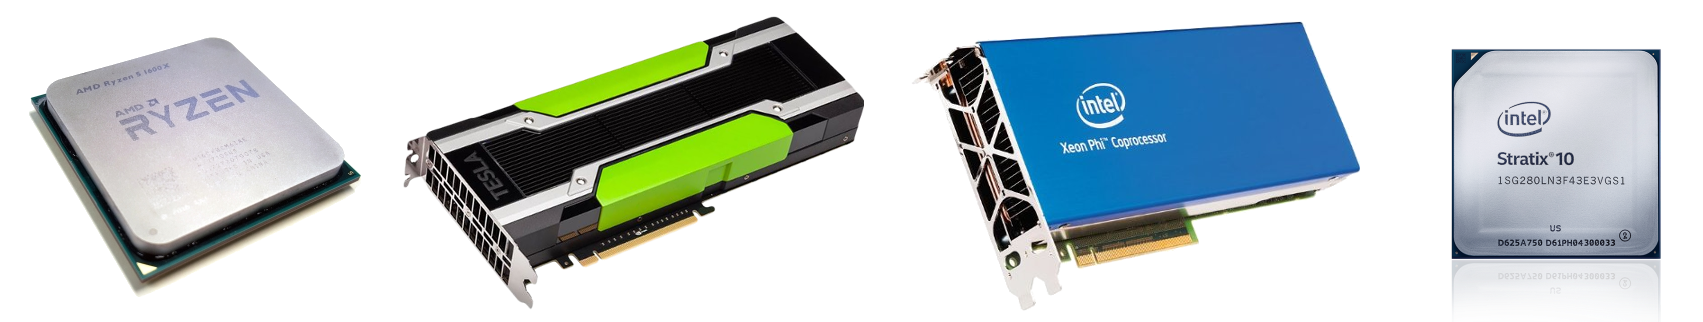
\includegraphics[width=\columnwidth]{architectures}
                \end{center}

                How to write \alert{efficient code} for each of these?
            \end{block}

            \begin{block}{Autotuning}

                \vspace{.2cm}

                The process of \alert{automatically finding} a
                \alert{configuration} of a program that optimizes an
                \alert{objective}
            \end{block}

        \column{.5\textwidth}
            \begin{block}{Configurations}
                \begin{itemize}
                    \item Program configuration
                        \begin{itemize}
                            \item Algorithm, block size, $\dots$
                                  %number of threads or processes
                        \end{itemize}
                    \item Source code transformation
                        \begin{itemize}
                            \item Loop unrolling, tiling, rotation, $\dots$
                        \end{itemize}
                    \item Compiler configuration
                        \begin{itemize}
                            \item \texttt{-O2}, vectorization, $\dots$
                                %register usage, instruction selection
                        \end{itemize}
                    \item $\dots$
                \end{itemize}
            \end{block}

            \begin{block}{Objectives}
                \begin{itemize}
                    \item Execution time
                    \item Memory \& power consumption
                    \item $\dots$
                \end{itemize}
            \end{block}

    \end{columns}
\end{frame}

\begin{frame}
    \frametitle{Autotuning: Search Spaces}
    \begin{columns}[c]
        \column{.49\textwidth}
            \begin{block}{Search Spaces}
                \vspace{.2cm}

                Represent the \alert{effect} of all possible
                \alert{configurations} on the \alert{objectives}

                Can be difficult to explore, with multiple \alert{local optima}
                and \alert{undefined regions}
            \end{block}

        \column{.49\textwidth}
            \begin{block}{}
                \begin{center}
                    %\includegraphics<1>[width=.75\columnwidth]{sample_search_space}
                    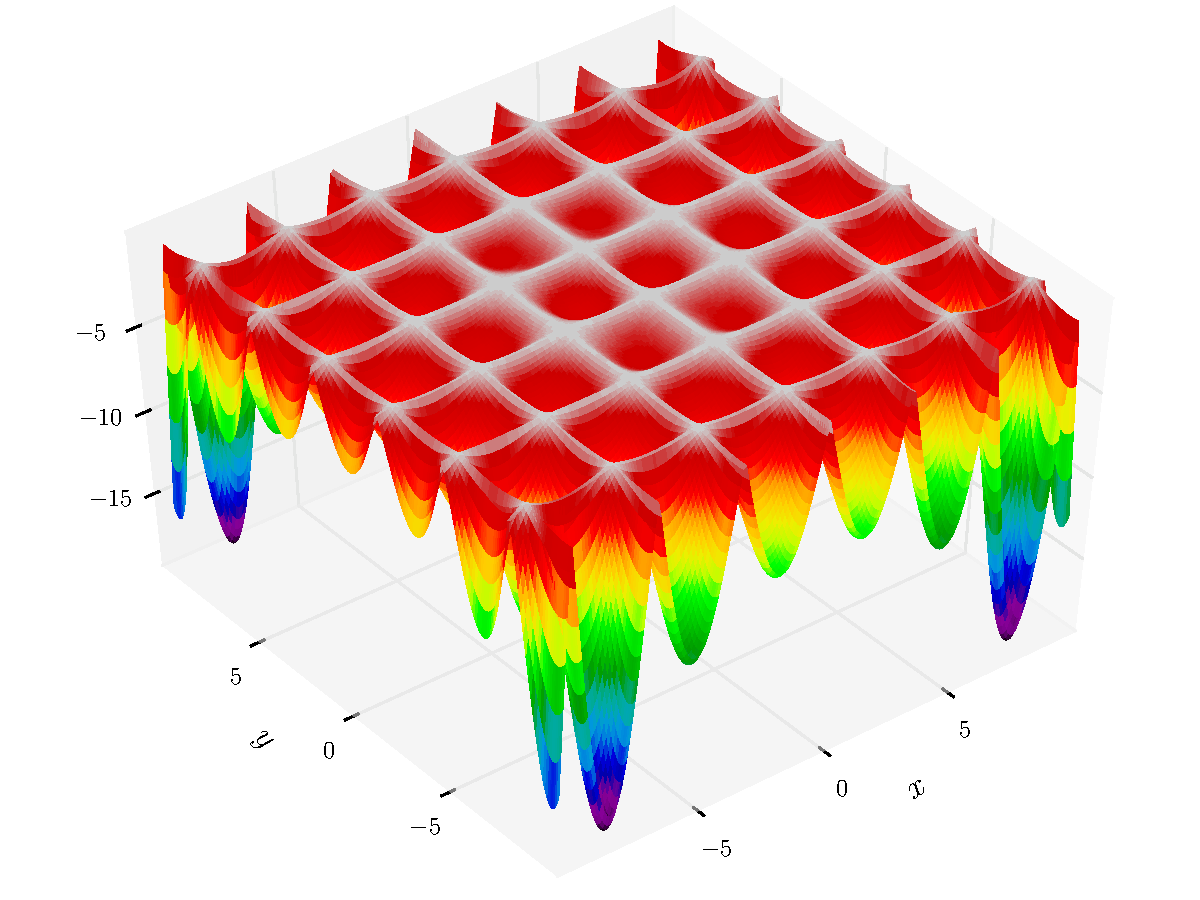
\includegraphics[width=.80\columnwidth]{holder_table}

                    %\only<1>{\alert{Mishra's Bird function}}
                    \alert{Hölder Table function}
                \end{center}
            \end{block}

    \end{columns}
\end{frame}

\begin{frame}
    \frametitle{Autotuning: Exploring Search Spaces}
    \begin{columns}[c]
        \column{.49\textwidth}
            \begin{block}{Issue 1: \alert{Exponential Growth}}
                \vspace{.2cm}

                \alert{Simple factors} can generate \alert{large spaces}:

                \begin{itemize}
                    \item 30 \textit{boolean} factors
                    \item $2^{30}$ combinations
                \end{itemize}
            \end{block}

            \begin{block}{Issue 2: \alert{Geometry}}
                \begin{itemize}
                    \item \alert{Discrete} or \alert{continuous} factors
                    \item \alert{``Smoothness''}
                    \item \alert{Interactions} between factors
                \end{itemize}
            \end{block}

        \column{.49\textwidth}
            \begin{block}{Issue 3: \alert{Measurement Time}}
                \vspace{.2cm}

                Time to \alert{compile}:

                \begin{itemize}
                    \item \alert{Benchmark} GPU applications:
                        \alert{1\textasciitilde10s}
                    \item \alert{Benchmark} FPGA applications:
                        \alert{1\textasciitilde10min}
                    \item \alert{Industrial} FPGA applications:
                        \alert{1\textasciitilde10h}
                \end{itemize}
            \end{block}

    \end{columns}
\end{frame}

\begin{frame}
    \frametitle{Autotuning: Multiple Approaches}
    \begin{columns}[c]
        \column{.49\textwidth}
            \begin{block}{Popular Approaches}
                \begin{itemize}
                    \item \footnotesize{\colorbox{red!25}{Exhaustive}}
                    \item \footnotesize{\colorbox{green!25}{Meta-Heuristics}}
                    \item \footnotesize{\colorbox{cyan!25}{Machine Learning}}
                \end{itemize}

                \vspace{-.4cm}

                \begin{table}
                    \centering
                    \scriptsize
                    \begin{tabular}{@{}lll@{}}
                        \toprule
                        System & Domain & Approach \\ \midrule
                        \rowcolor{red!25} ATLAS & Dense Linear Algebra & Exhaustive\\ \addlinespace
                        \rowcolor{green!25} INSIEME & Compiler & Genetic Algorithm \\
                        \rowcolor{green!25} Active Harmony & Runtime & Nelder-Mead \\
                        \rowcolor{green!25} ParamILS & Domain-Agnostic & Stochastic Local Search \\
                        \rowcolor{green!25} OPAL & Domain-Agnostic & Direct Search \\
                        \rowcolor{green!25} OpenTuner & Domain-Agnostic & Ensemble \\ \addlinespace
                        \rowcolor{cyan!25} MILEPOST GCC & Compiler & Machine Learning \\
                        \rowcolor{cyan!25} Apollo & GPU kernels & Decision Trees \\ \addlinespace
                        \bottomrule
                    \end{tabular}
                \end{table}
            \end{block}

        \column{.49\textwidth}
            \begin{block}{Main Issues}
                \begin{itemize}
                    \item These approaches \alert{assume}:
                        \begin{itemize}
                            \item A \alert{large number of function evaluations}
                            \item Search space \alert{``smoothness''}
                            \item Good solutions are \alert{reachable}
                        \end{itemize}
                    \item After optimizing:
                        \begin{itemize}
                            \item \alert{Learn nothing} about the search space
                            \item \alert{Can't explain} why optimizations work
                        \end{itemize}
                \end{itemize}
            \end{block}

    \end{columns}
\end{frame}

\section{Applying Design of Experiments to Autotuning}

\begin{frame}
    \frametitle{Applying Design of Experiments to Autotuning}
    \begin{columns}[c]
        \column{.49\textwidth}
            \begin{block}{Our Approach}

                \vspace{.2cm}

                Using \alert{efficient experimental designs} to overcome issues
                related to \alert{exponential growth}, \alert{geometry}, and
                \alert{measurement time}
            \end{block}

            \begin{block}{Design Requirements}
                \begin{itemize}
                    \item Support a large number of factors (\alert{Exponential Growth})
                    \item Support continous and discrete factors (\alert{Geometry})
                    \item Minimize function evaluations (\alert{Measurement Time})
                \end{itemize}
            \end{block}

        \column{.49\textwidth}
            \begin{block}{Main Design Candidates}

                \vspace{.2cm}

                \alert{Screening} Designs:

                \begin{itemize}
                    \item Estimate \alert{main effects}
                    \item Aim to \alert{minimize runs}
                    \item Assume \alert{interactions are negligible}
                \end{itemize}

                \alert{Mixed-Level} Designs:

                \begin{itemize}
                    \item Factors have \alert{different number of levels}
                    \item Many \alert{optimality criteria}
                \end{itemize}

            \end{block}

    \end{columns}
\end{frame}

\begin{frame}
    \frametitle{Screening Designs}
    \begin{columns}[c]
        \column{.49\textwidth}
            \vspace{.4cm}

            A Plackett-Burman \alert{screening design} for $7$
            \alert{$2$-level factors}:

            \vspace{.2cm}

            \begin{table}[]
                \centering
                \begin{tabular}{@{}cccccccc@{}}
                    \toprule
                    Run & A & B & C & D & E & F & G \\ \midrule
                    \cellcolor{gray!18}1 & \cellcolor{green!25}1 & \cellcolor{red!25}-1 & \cellcolor{green!25}1 & \cellcolor{red!25}-1 & \cellcolor{red!25}-1 & \cellcolor{green!25}1 & \cellcolor{green!25}1 \\
                    \cellcolor{gray!18}2 & \cellcolor{green!25}1 & \cellcolor{green!25}1 & \cellcolor{green!25}1 & \cellcolor{red!25}-1 & \cellcolor{green!25}1 & \cellcolor{red!25}-1 & \cellcolor{red!25}-1 \\
                    \cellcolor{gray!18}3 & \cellcolor{red!25}-1 & \cellcolor{green!25}1 & \cellcolor{red!25}-1 & \cellcolor{red!25}-1 & \cellcolor{green!25}1 & \cellcolor{green!25}1 & \cellcolor{green!25}1 \\
                    \cellcolor{gray!18}4 & \cellcolor{red!25}-1 & \cellcolor{green!25}1 & \cellcolor{green!25}1 & \cellcolor{green!25}1 & \cellcolor{red!25}-1 & \cellcolor{green!25}1 & \cellcolor{red!25}-1 \\
                    \cellcolor{gray!18}5 & \cellcolor{green!25}1 & \cellcolor{red!25}-1 & \cellcolor{red!25}-1 & \cellcolor{green!25}1 & \cellcolor{green!25}1 & \cellcolor{green!25}1 & \cellcolor{red!25}-1 \\
                    \cellcolor{gray!18}6 & \cellcolor{green!25}1 & \cellcolor{green!25}1 & \cellcolor{red!25}-1 & \cellcolor{green!25}1 & \cellcolor{red!25}-1 & \cellcolor{red!25}-1 & \cellcolor{green!25}1 \\
                    \cellcolor{gray!18}7 & \cellcolor{red!25}-1 & \cellcolor{red!25}-1 & \cellcolor{green!25}1 & \cellcolor{green!25}1 & \cellcolor{green!25}1 & \cellcolor{red!25}-1 & \cellcolor{green!25}1 \\
                    \cellcolor{gray!18}8 & \cellcolor{red!25}-1 & \cellcolor{red!25}-1 & \cellcolor{red!25}-1 & \cellcolor{red!25}-1 & \cellcolor{red!25}-1 & \cellcolor{red!25}-1 & \cellcolor{red!25}-1  \\ \bottomrule
                \end{tabular}
            \end{table}

        \column{.49\textwidth}
            \begin{block}{Screening Designs}

                \vspace{.2cm}

                \alert{Plackett-Burman} designs for \alert{2-level factors}:

                \begin{itemize}
                    \item \alert{Orthogonal arrays} of \alert{strength 2}
                    \item Estimate the \alert{main effects} of \alert{$n$
                        factors with $n + 1$ runs}
                \end{itemize}

                Construction:

                \begin{itemize}
                    \item For \alert{$n + 1$ multiple of $4$}
                    \item Identical to a fractional factorial design if
                        \alert{$n + 1$ is a power of two}
                \end{itemize}
            \end{block}

    \end{columns}
\end{frame}

\begin{frame}
    \frametitle{Looking at Data: CUDA Compiler Flags}
    \begin{columns}[c]
        \column{.35\textwidth}
            \begin{block}{CUDA Compiler Flags}
                \begin{itemize}
                    \item \alert{Rodinia Benchmark}
                    \item \alert{15} factors, \alert{few with
                        multiple levels}
                    \item \alert{$10^6$} combinations
                    \item \alert{$1$\textasciitilde$10$s} to measure
                    \item \alert{Screening Experiment}:
                        \begin{itemize}
                            \item \alert{15 ``2-level''} factors
                            \item \alert{4 ``dummy''} factors
                        \end{itemize}
                \end{itemize}
            \end{block}

        \column{.65\textwidth}
            \begin{block}{}
                \vspace{-.4cm}
                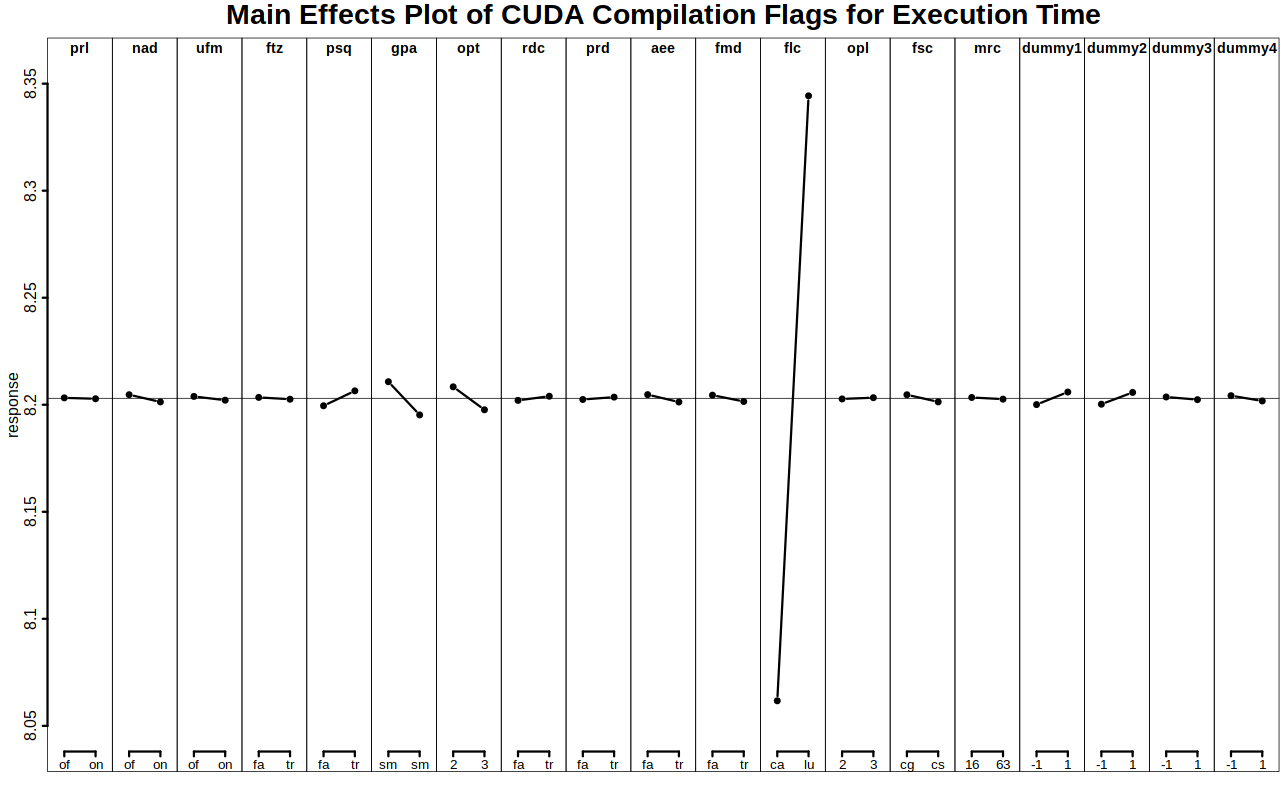
\includegraphics[width=.98\textwidth]{main_effects_gpu}
            \end{block}

    \end{columns}
\end{frame}

\begin{frame}
    \frametitle{Mixed-Level Designs}
    \begin{columns}[c]
        \column{.49\textwidth}

            \vspace{.1cm}

            A \alert{multi-level} design for $1$ \alert{$2$-level factor}
            and $3$ \alert{$3$-level factors}:

            \vspace{-.3cm}

            \begin{table}[]
                \scriptsize
                \centering
                \begin{tabular}{@{}ccccc@{}}
                    \toprule
                    Run & A & B & C & D \\ \midrule
                    \cellcolor{gray!18}1 & \cellcolor{green!25}1 & \cellcolor{green!25}1 & \cellcolor{green!25}1 & \cellcolor{red!25}3 \\
                    \cellcolor{gray!18}2 & \cellcolor{green!25}1 & \cellcolor{green!25}1 & \cellcolor{cyan!25}2 & \cellcolor{green!25}1 \\
                    \cellcolor{gray!18}3 & \cellcolor{green!25}1 & \cellcolor{green!25}1 & \cellcolor{red!25}3 & \cellcolor{cyan!25}2 \\
                    \cellcolor{gray!18}4 & \cellcolor{green!25}1 & \cellcolor{cyan!25}2 & \cellcolor{green!25}1 & \cellcolor{cyan!25}2 \\
                    \cellcolor{gray!18}5 & \cellcolor{green!25}1 & \cellcolor{cyan!25}2 & \cellcolor{cyan!25}2 & \cellcolor{red!25}3 \\
                    \cellcolor{gray!18}6 & \cellcolor{green!25}1 & \cellcolor{cyan!25}2 & \cellcolor{red!25}3 & \cellcolor{green!25}1 \\
                    \cellcolor{gray!18}7 & \cellcolor{green!25}1 & \cellcolor{red!25}3 & \cellcolor{green!25}1 & \cellcolor{green!25}1 \\
                    \cellcolor{gray!18}8 & \cellcolor{green!25}1 & \cellcolor{red!25}3 & \cellcolor{cyan!25}2 & \cellcolor{cyan!25}2 \\
                    \cellcolor{gray!18}9 & \cellcolor{green!25}1 & \cellcolor{red!25}3 & \cellcolor{red!25}3 & \cellcolor{red!25}3 \\
                    \cellcolor{gray!18}10 & \cellcolor{cyan!25}2 & \cellcolor{green!25}1 & \cellcolor{green!25}1 & \cellcolor{green!25}1 \\
                    \cellcolor{gray!18}11 & \cellcolor{cyan!25}2 & \cellcolor{green!25}1 & \cellcolor{cyan!25}2 & \cellcolor{cyan!25}2 \\
                    \cellcolor{gray!18}12 & \cellcolor{cyan!25}2 & \cellcolor{green!25}1 & \cellcolor{red!25}3 & \cellcolor{red!25}3 \\
                    \cellcolor{gray!18}13 & \cellcolor{cyan!25}2 & \cellcolor{cyan!25}2 & \cellcolor{green!25}1 & \cellcolor{red!25}3 \\
                    \cellcolor{gray!18}14 & \cellcolor{cyan!25}2 & \cellcolor{cyan!25}2 & \cellcolor{cyan!25}2 & \cellcolor{green!25}1 \\
                    \cellcolor{gray!18}15 & \cellcolor{cyan!25}2 & \cellcolor{cyan!25}2 & \cellcolor{red!25}3 & \cellcolor{cyan!25}2 \\
                    \cellcolor{gray!18}16 & \cellcolor{cyan!25}2 & \cellcolor{red!25}3 & \cellcolor{green!25}1 & \cellcolor{cyan!25}2 \\
                    \cellcolor{gray!18}17 & \cellcolor{cyan!25}2 & \cellcolor{red!25}3 & \cellcolor{cyan!25}2 & \cellcolor{red!25}3 \\
                    \cellcolor{gray!18}18 & \cellcolor{cyan!25}2 & \cellcolor{red!25}3 & \cellcolor{red!25}3 & \cellcolor{green!25}1 \\ \bottomrule
                \end{tabular}
            \end{table}


        \column{.49\textwidth}
            \begin{block}{Mixed-Level Designs}

                \vspace{.2cm}

                \textbf{Strategy 1: \alert{Contractive Replacement}}

                \begin{itemize}
                    \item Find \alert{specific sets of $k$-level columns} of a
                        design, \alert{contract} the set into a new
                        \alert{factor with more levels}
                    \item \alert{Maintain orthogonality} of the design
                \end{itemize}

                \textbf{Strategy 2: \alert{Direct Construction}}

                Directly generate \alert{small mixed-level designs} by
                solving \alert{Mixed Integer Programming problems}

                \textbf{Strategy 3: \alert{D-Optimal Designs}}
            \end{block}

    \end{columns}
\end{frame}

\begin{frame}
    \frametitle{D-Optimal Designs}
    \begin{columns}[c]
        \column{.49\textwidth}
            \begin{block}{Construction}
                \begin{itemize}
                    \item Define \alert{factors and levels}
                    \item Choose a \alert{model}
                    \item Choose an \alert{optimality metric}
                    \item \alert{Select} runs from the \alert{full factorial
                        design}
                \end{itemize}
            \end{block}

        \column{.49\textwidth}
            \begin{block}{Example}
                \begin{itemize}
                    \item Factors: $x_1 = \{-1, 0, 1\}, x_2 = \{-1, 0, 1\}$
                    \item Model: $\mathbf{Y} = \mathbf{X}\beta + \eta$
                    \item Choose an \alert{optimality metric}
                    \item \alert{Select} runs from the \alert{full factorial
                        design}
                \end{itemize}
            \end{block}

    \end{columns}
\end{frame}

\begin{frame}
    \frametitle{Looking at Data: FPGA Compiler Parameters}
    \begin{columns}[c]
        \column{.4\textwidth}
            \begin{block}{FPGA Compiler Parameters}
                \begin{itemize}
                    \item \alert{CHStone Benchmark}
                    \item \alert{141} factors, \alert{most with multiple
                        levels}
                    \item \alert{$10^{128}$} combinations
                    \item \alert{$1$\textasciitilde$10$min} to measure
                    \item \alert{Multiple objectives}
                    \item \alert{Search with Meta-Heuristics}:
                        \begin{itemize}
                            \item \alert{Unstructured data difficults analysis}
                            \item We are working on \alert{obtaining more data}
                        \end{itemize}
                \end{itemize}
            \end{block}

        \column{.6\textwidth}
            \begin{block}{}
                \vspace{-.4cm}
                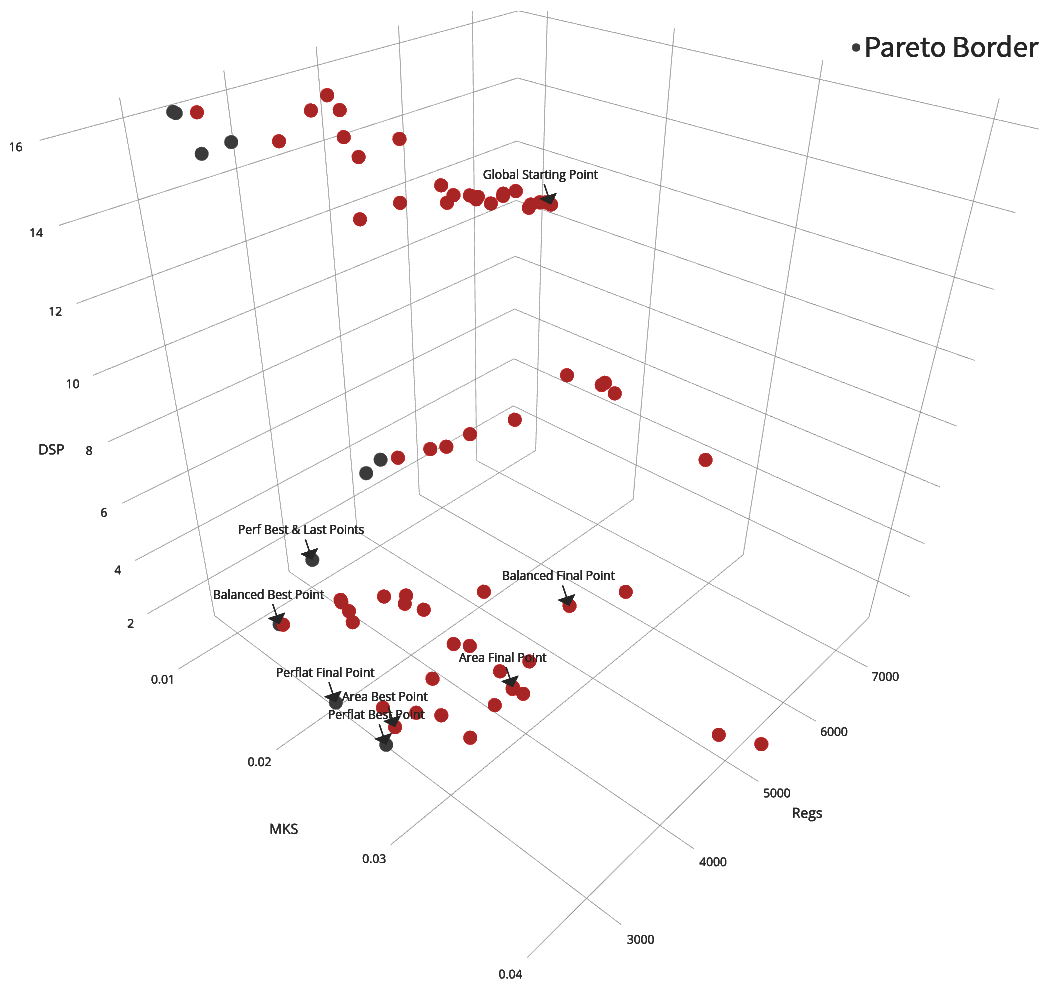
\includegraphics[width=.8\textwidth]{fpga_space}
            \end{block}

    \end{columns}
\end{frame}

\section{Perspectives}

\begin{frame}
    \frametitle{Perspectives}
    \begin{columns}[c]
        \column{.5\textwidth}
            \begin{block}{Perspectives}
                \begin{itemize}
                    \item \alert{Short term}:
                        \begin{itemize}
                            \item Study \alert{small}, \alert{balanced},
                                \alert{orthogonal} \alert{multi-level} designs
                                for \alert{large numbers of factors}
                            \item Iteratively \alert{drop least significant
                                factors} with \alert{user input}
                        \end{itemize}
                    \item \alert{Long term}:
                        \begin{itemize}
                            \item Use such designs to \alert{autotune
                                industrial-level FPGA applications}
                            \item Provide an \alert{autotuning shared library}
                                to applications
                        \end{itemize}
                \end{itemize}
            \end{block}

        \column{.5\textwidth}
            \begin{block}{Takeaway}

                \vspace{.2cm}

                \textbf{Target Scenario: \alert{FPGA Compiler Parameters}}

                \vspace{-.1cm}

                \begin{itemize}
                    \item \alert{Large search space}
                    \item \alert{Large measurement time}
                    \item Factors with \alert{multiple levels}
                \end{itemize}

                \vspace{-.1cm}

                \textbf{Our Approach}

                Using \alert{efficient experimental designs} to overcome issues
                related to \alert{exponential growth}, \alert{geometry}, and
                \alert{measurement time}

                \textbf{Main Design Candidates}

                \alert{Screening} \& \alert{Mixed-Level} designs

            \end{block}

    \end{columns}
\end{frame}

\maketitle

\end{document}
